% !TeX root = RJwrapper.tex 
\title{A Computational Analysis of the Dynamics of R Style Based on 108 Million Lines of Code from All CRAN Packages in the Past 21 Years}
\author{by Chia-Yi Yen, Mia Huai-Wen Chang, Chung-hong Chan}

\maketitle

\abstract{
The flexibility of R and the diversity of the R community leads to a large number of programming styles applied in R packages. We have analyzed 108 million lines of R code from CRAN and quantified the evolution in popularity of 12 style-elements from 1998 to 2019. We attribute 3 main factors that drive changes in programming style: the effect of style-guides, the effect of introducing new features, and the effect of editors. We observe in the data that a consensus in programming style is forming, e.g. snake case, use <- for assignment.
\footnote{
    We have presented a previous version of this paper as a poster at UseR! 2019 Toulouse. Interested readers can access it with the following link: \url{
    https://github.com/chainsawriot/rstyle/blob/master/docs/Poster_useR2019_Toulouse.png}
}
}

\section{Introduction}

R is flexible. For example, one can use \code{<-} or \code{=} as assignment operators. The following two functions can both be correctly evaluated.

\begin{example}
sum_of_square <- function(x) {
    return(sum(x^2))
}
\end{example}

\begin{example}
sum_oF.square=function(x)
{
    sum(x ^ 2)}
\end{example}

One area that can highlight this flexibility is naming conventions. According to the previous research by \citet{baaaath}, there are at least 6 styles and none of the 6 has dominated the scene. Beyond naming conventions investigated by \citet{baaaath}, there are style-elements that R programmers have the freedom to adopt, e.g. whether or not to add spaces around infix operators, use double quotation marks or single quotation marks to denote strings. On one hand, these variations provide programmers with freedom. On the other hand, these variations can confuse new programmers and can have dire effects on program comprehension. Also, incompatibility between programming styles might also affect reusability, maintainability \citep{elish}, and open source collaboration \citep{wang}. 

Various efforts to standardize the programming style, e.g. Google's R Style Guide \citep{google}, the Tidyverse Style Guide \citep{tidyverse}, Bioconductor Coding Style \citep{bioconductor},  are available (Table~\ref{tab:table1}) \footnote{\citet{baaaath} lists also \href{https://csgillespie.wordpress.com/2010/11/23/r-style-guide/}{Colin Gillespie's R style guide}.  Additional style guides that we found include the style guides by \href{https://docs.google.com/document/d/1esDVxyWvH8AsX-VJa-8oqWaHLs4stGlIbk8kLc5VlII/edit}{Henrik Bengtsson}, \href{https://jef.works/R-style-guide/}{Jean Fan}, \href{https://irudnyts.github.io//r-coding-style-guide/}{Iegor Rudnytskyi}, \href{https://rpahl.github.io/r-some-blog/my-r-style-guide/}{Roman Pahl}, \href{https://cran.r-project.org/web/packages/rockchalk/vignettes/Rstyle.pdf}{Paul E. Johnson}, \href{https://bookdown.org/joshuah40/qa_code/Coding-Guidelines.html}{Joshua Halls},  \href{https://www.datanovia.com/en/blog/r-coding-style-best-practices/}{Datanovia}, and \href{https://www.daqana.org/dqstyle-r/}{daqana}. We focus only on the 3 style guides of Tidyverse, Google and Bioconductor is because these 3 are arguably the most influential. There are groups of developers (e.g. contributors to \CRANpkg{tidyverse}, Google employees, and Bioconductor contributors) adhering to these 3 styles.}.

Among the 3 style-guides, the major differences are the suggested naming convention and indentation, as highlighted in Table~\ref{tab:table1}. Other style-elements are essentially the same. These style guides are based on possible improvement in code quality, e.g. style-elements that improve program comprehension \citep{oman}. However, we argue that one should first study the current situation, and preferably, the historical development, of programming style variations (PSV) to supplement these standardization efforts. We have undertaken such a task, so that the larger R communities can have a baseline to evaluate the effectiveness of those standardization efforts. Also, we can have a better understanding of the factors driving increase and decrease in PSV historically, such that more effective standardization efforts can be formulated.

\newcolumntype{L}{>{\centering\arraybackslash}m{3cm}}

\begin{table}

\caption{\label{tab:table1}Three major style-guides: Google, Tidyverse and Bioconductor}
\centering
\begin{tabular}[t]{L|L|L|L}
\hline
Feature & Google & Tidyverse & Bioconductor\\
\hline
\textbf{Function name} & UpperCamel & snake\_case & lowerCamel\\
\hline
Assignment & Discourage = & Discourage = & Discourage =\\
\hline
Line length & “limit your code to 80 characters per line” & “limit your code to 80 characters per line” & $\leqslant$ 80\\
\hline
Space after a comma & Yes & Yes & Yes\\
\hline
Space around infix operators & Yes & Yes & Yes\\
\hline
\textbf{Indentation} & 2 spaces & 2 spaces & 4 spaces\\
\hline
Integer & Not specified & Not specified (Integers are not explicitly typed in included code examples) & Not specified\\
\hline
Quotes & Double & Double & Not specified\\
\hline
Boolean values & Use TRUE / FALSE & Use TRUE / FALSE & Not specified\\
\hline
Terminate a line with a semicolon & No & No & Not specified\\
\hline
Curly braces & \{ same line, then a newline, \} on its own line & \{ same line, then a newline, \} on its own line & Not specified\\
\hline
\end{tabular}
\end{table}


\section{Analysis}
\subsection{Data Source}

On July 1, 2020, we cloned a local mirror of CRAN using the rsync method suggested in the CRAN Mirror HOWTO \citep{cranminihowto}. Our local mirror contains all contributed packages as tarball files (.tar.gz). By all contributed packages, we mean packages actively listed online on the CRAN website as well as orphaned and archived packages. In this analysis, we include all active, orphaned and archived packages.

In order to facilitate the analysis, we have developed the package \code{baaugwo} \citep{chan2} to extract all R source code and metadata from these tarballs. In this study, only the source code from the \code{/R} directory of each tarball file is included. We have also archived the metadata from the \code{DESCRIPTION} and \code{NAMESPACE} files from the tarballs.

In order to cancel out the over-representation effect of multiple submissions in a year by a particular package, we have applied the \emph{"one-submission-per-year"} rule to randomly selected only one submission from a year for each package. Unless otherwise noticed, we present below the analysis of this \emph{"one-submission-per-year"} sample. Similarly, unless otherwise noticed, the unit of the analysis is \emph{exported function}. The study period for this study is from 1998 to 2019.

\subsection{Quantification of PSV}

All exported functions in our sample are parsed into a parse tree using the parser from the \CRANpkg{lintr} \citep{lintr} package.

These parse trees were then filtered for lines with function definition and then linted them using the linters from the lintr package to detect for various style-elements. Style-elements considered in this study are:

\paragraph{fx\_assign}

Use = as assignment operators

\begin{example}
softplusFunc = function(value, leaky = FALSE) {
    if (leaky) {
        warnings("using leaky RELU!")
        return(ifelse(value > 0L, value, value * 0.01))
    }
    return(log(1L + exp(value)))
}
\end{example}

\paragraph{fx\_opencurly}

An open curly is on its own line

\begin{example}
softplusFunc <- function(value, leaky = FALSE) 
{
    if (leaky) 
    {
        warnings("using leaky RELU!")
        return(ifelse(value > 0L, value, value * 0.01))
    }
    return(log(1L + exp(value)))
}
\end{example}

\paragraph{fx\_infix}

No spaces are added around infix operators.

\begin{example}
softplusFunc<-function(value, leaky=FALSE) {
    if (leaky) {
        warnings("using leaky RELU!")
        return(ifelse(value>0L, value, value*0.01))
    }
    return(log(1L+exp(value)))
}
\end{example}

\paragraph{fx\_integer}

Not explicitly type integers

\begin{example}
softplusFunc <- function(value, leaky = FALSE) {
    if (leaky) {
        warnings("using leaky RELU!")
        return(ifelse(value > 0, value, value * 0.01))
    }
    return(log(1 + exp(value)))
}
\end{example}

\paragraph{fx\_singleq}

Use single quotation marks for strings

\begin{example}
softplusFunc <- function(value, leaky = FALSE) {
    if (leaky) {
        warnings('using leaky RELU!')
        return(ifelse(value > 0L, value, value * 0.01))
    }
    return(log(1L + exp(value)))
}
\end{example}

\paragraph{fx\_commas}

No space is added after commas

\begin{example}
softplusFunc <- function(value,leaky = FALSE) {
    if (leaky) {
        warnings("using leaky RELU!")
        return(ifelse(value > 0L,value,value * 0.01))
    }
    return(log(1L + exp(value)))
}
\end{example}

\paragraph{fx\_semi}

Use semicolons to terminate lines

\begin{example}
softplusFunc <- function(value, leaky = FALSE) {
    if (leaky) {
        warnings("using leaky RELU!");
        return(ifelse(value > 0L, value, value * 0.01));
    }
    return(log(1L + exp(value)));
}
\end{example}

\paragraph{fx\_t\_f}

Use T/F instead of TRUE / FALSE

\begin{example}
softplusFunc <- function(value, leaky = F) {
    if (leaky) {
        warnings("using leaky RELU!")
        return(ifelse(value > 0L, value, value * 0.01))
    }
    return(log(1L + exp(value)))
}
\end{example}

\paragraph{fx\_closecurly}

An close curly is not on its own line.

\begin{example}
softplusFunc <- function(value, leaky = FALSE) {
    if (leaky) {
        warnings("using leaky RELU!")
        return(ifelse(value > 0L, value, value * 0.01)) }
    return(log(1L + exp(value))) }
\end{example}

\paragraph{fx\_tab}

Use tab to indent

\begin{example}
softplusFunc <- function(value, leaky = FALSE) {
    if (leaky) {
        warnings("using leaky RELU!")
        return(ifelse(value > 0L, value, value * 0.01))
    }
    return(log(1L + exp(value)))
}
\end{example}

We have studied also the naming conventions of all included functions. Using the similar technique of \citet{baaaath}, we classified function names into the following 7 categories:

\begin{itemize}
  \item \textbf{alllower} softplusfunc
  \item \textbf{ALLUPPER} SOFTPLUSFUNC
  \item \textbf{UpperCamel} SoftPlusFunc
  \item \textbf{lowerCamel} softPlusFunc
  \item \textbf{lower\_snake} soft\_plus\_func
  \item \textbf{dotted.func} soft.plus.func
  \item \textbf{other} sOfTPluSfunc
\end{itemize}

The last style-element is line-length. For each R file, we counted the distribution of line-length. In this analysis, the unit of analysis is line.

If not considering line-length, the remaining 10 binary and one multinomial leave 7,168 possible combinations of PSVs that a programmer could employ ($7 \times 2^{10} = 7,168$).

\subsection{Methodology of community-specific variations analysis}

On top of the overall patterns based on the analysis of all functions, the community-specific variations are also studied. In this part of the study, we ask the question: do local patterns of PSV exist in various programming communities? To this end, we constructed a dependency graph of CRAN packages by defining a package as a node and an import/suggest relationship as a directed edge. Communities in this dependency graph were extracted using the Walktrap Community Detection Algorithm \citep{pons} provided by the \CRANpkg{igraph} package \citep{csardi}. The step parameter was set at 4 for this analysis. Notably, we analyzed the dependency graph as a snapshot, which is built based on the submission history of every package from 1998 to 2019. 

By applying the Walktrap Community Detection on the 2019 data, we have identified 931 communities in this CRAN dependency graph. The purpose of this analysis is to show the PSV in different communities. We selected the largest 20 communities for further analysis. The choice of 20 is deemed enough to show these community-specific variations. These 20 identified communities cover 88\% of the total 14,491 packages, which shows that the coverage of our analysis is comprehensive. Readers could explore other choices themselves using our openly shared data.

\subsection{Methodology of within-package variations analysis}

Maintaining a consistent style in source code can enable efficient reading by multiple readers \citep{gillespie2016efficient} \footnote{Maintaining a consistent style is even thought to be a quality of a successful R programmer in \citet{gillespie2016efficient}.}. In addition to community-level analysis, we extend our work to the package-level, in which we investigate the consistency of different style elements within a package. In this analysis, we studied 12 style elements, including fx\_assign, fx\_commas, fx\_integer, fx\_semi, fx\_t\_f, fx\_closecurly, fx\_infix, fx\_opencurly, fx\_singleq, fx\_tab, and fx\_name.  In other words, 11 binary variables (the first 11) and 1 multinomial variable (fx\_name) could be assigned to each function within a package.

We quantified the package-level consistency by computing the entropy for each style element. Given a style element S of an R package $R_{i}$, with possible n choices $s_{1}$, $\mathellipsis$ $s_{n}$ (e.g. n = 2 for binary; n = 7 for fx\_names), the entropy $H(S)$ is calculated as:

\begin{equation} \label{eqn}
H(S) = - \sum_{i = 1}^{n} P(s_{i}) \log P(s_{i})
\end{equation}

$P(s_{i})$ is calculated as the proportion of all functions in $R_{i}$ with the style element $s_{i}$. For example, if a package has 4 functions and the S of these 4 functions are {0,0,1,2}. The entropy $H(S)$ is $- ((0.5 \times log(0.5)) + (0.25 \times log(0.25)) + (0.25 \times log(0.25))) = 0.45$.

As the value of $H(S)$ is not comparable across different S with a different number of n, we normalize the value of $H(S)$ into $H'(S)$ by dividing $H(S)$ with the theoretical maximum. The maximum values of $H(S)$ for n = 2 and n = 7 are 0.693 and 1.946, respectively.

Finally, we calculate the $\bar{H'(S)}$ of all CRAN packages (i.e. $R_{1}$ $\mathellipsis$ $R_{n}$, where n equals the number of all CRAN packages) by averaging the $H'(S)$.

\section{Results}

We studied more than 108 million lines of code from 17,692 unique packages. In total, 2,249,326 exported functions were studied. Figure~\ref{figure:fig1} displays the popularity of the 10 binary style-elements from 1998 to 2019. Some style-elements have very clear trends towards a majority-vs-minority pattern, e.g. fx\_closecurly, fx\_semi, fx\_t\_f and fx\_tab. Some styles-elements are instead trending towards a divergence from a previous majority-vs-minority pattern, e.g. fx\_assign, fx\_commas, fx\_infix, fx\_integer, fx\_opencurly and fx\_singleq. There are two style-elements that deserve special scrutiny. Firstly, the variation in fx\_assign is an illustrative example of the effect of introducing a new language feature by the R Development Core Team. The introduction of the language feature (= as assignment operator) in R 1.4 \citep{chambers} has coincided with the taking off in popularity of such style-element since 2001. Up to now, around 20\% of exported functions use such style.

\begin{figure}[htbp]
  \centering
  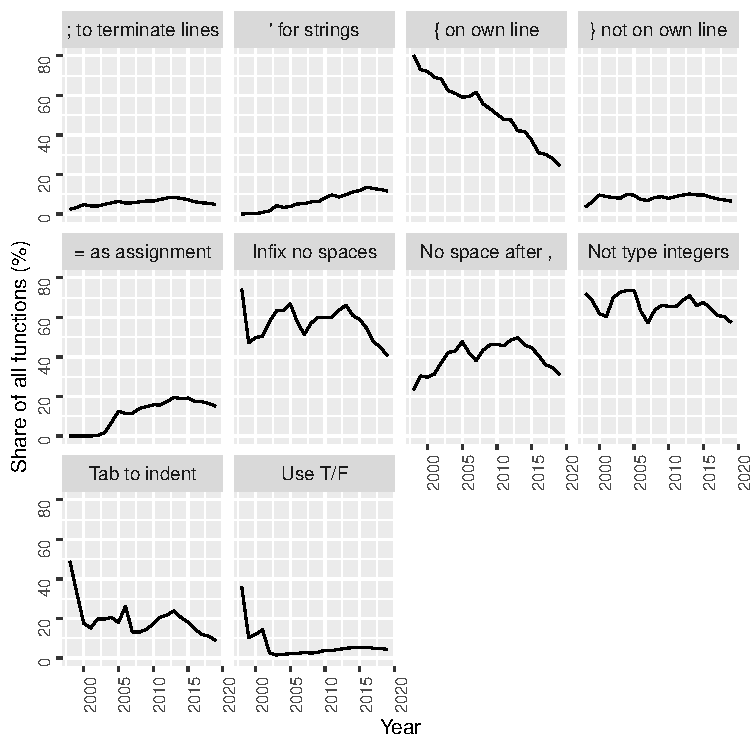
\includegraphics{fig1}
  \caption{Evolution in popularity of 10 style-elements from 1998 to 2019.}
  \label{figure:fig1}
\end{figure}


Secondly, the popularity of fx\_opencurly shows how a previously established majority style (~80\% in late 90s) slowly reduced into a minority, but still prominent, style (~30\% in late 10s).

Similarly, the evolution of different naming conventions is shown in Figure~\ref{figure:fig2} \footnote{'Other' is the 4th most popular naming convention. Some examples of function names classified as 'other' are: \emph{Blanc-Sablon}, \emph{returnMessage.maxim}, \emph{table\_articles\_byAuth}, \emph{mktTime.market}, \emph{smoothed\_EM}, \emph{plot.Sncf2D}, \emph{as.igraph.EPOCG}, \emph{TimeMap.new}, \emph{fT.KB}, \emph{IDA\_stable}. These functions were classified as 'other' because of the placement of capital letters. For packages using an all capitals object class name (e.g. EPOCG) and S3 generic method names (e.g. as.igraph), their methods are likely to be classified as 'others'. One could also classify these functions as dotted.func. However, we follow both \CRANpkg{lintr} and \citet{baaaath} to classify a function as dotted.func only when no capital letter is used in its name.}. This analysis can best be used to illustrate the effect of style-guides. According to \citet{baaaath}, dotted.func style is very specific to R programming. This style is the most dominant style in the early days of CRAN. However, multiple style guides advise against the use of dotted.func style and thus a significant declining trend is observed. lower\_snake and UpperCamel are the styles endorsed by the Tidyverse Style Guide and the Google's R Style Guide, respectively. These two styles see an increasing trend since the 2010s, while the growth of lower\_snake is stronger, with almost a 20\% growth in the share of all functions in contrast with the 1-2\% growth of other naming conventions. In 2019, lower\_snake (a style endorsed by Tidyverse) is the most popular style (26.6\%). lowerCamel case, a style endorsed by Bioconductor, is currently the second most popular naming convention (21.3\% in 2019). Only 7.0\% of functions use UpperCamel, the style endorsed by Google.

\begin{figure}[htbp]
  \centering
  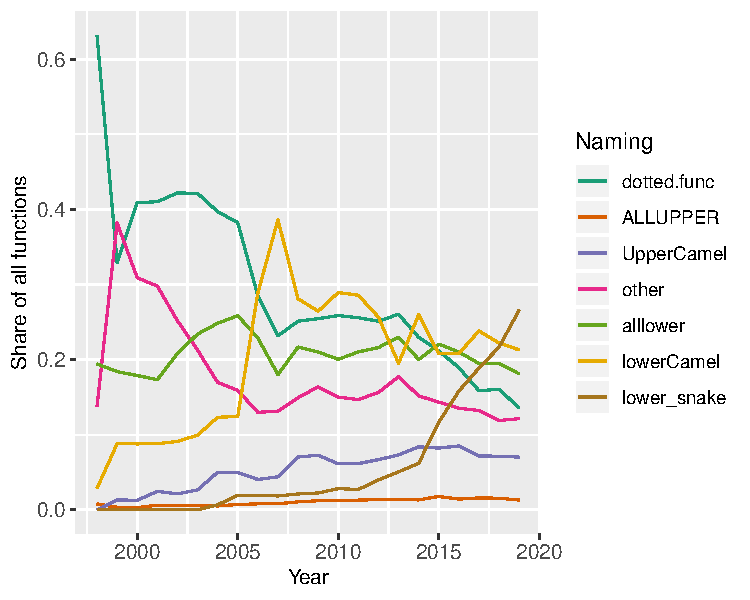
\includegraphics{fig2}
  \caption{Evolution in popularity of 7 naming conventions from 1998 to 2019.}
  \label{figure:fig2}
\end{figure}

The evolution of line lengths is tricky to be visualized on a 2-D surface. We have prepared a Shiny app (\url{https://chung-hong-chan.shinyapps.io/shiny/}) to visualize the change in line distribution over the span of 20 years. In this paper, Figure~\ref{figure:fig3} shows the snapshot of the change in line length distribution in the range of 40 to 100 characters. In general, developers of newer packages write with less characters per line. Similar to previous analyses with Python programs e.g.\citet{vanderplas}, artificial peaks corresponding to recommendations from either style-guides, linters, and editor settings are also observed in our analysis. In 2019, the artificial peak of 80 characters (recommended by most of the style-guides and linters such as \CRANpkg{lintr}) is more pronounced for lines with comments but not those with actual code.

\begin{figure}[htbp]
  \centering
  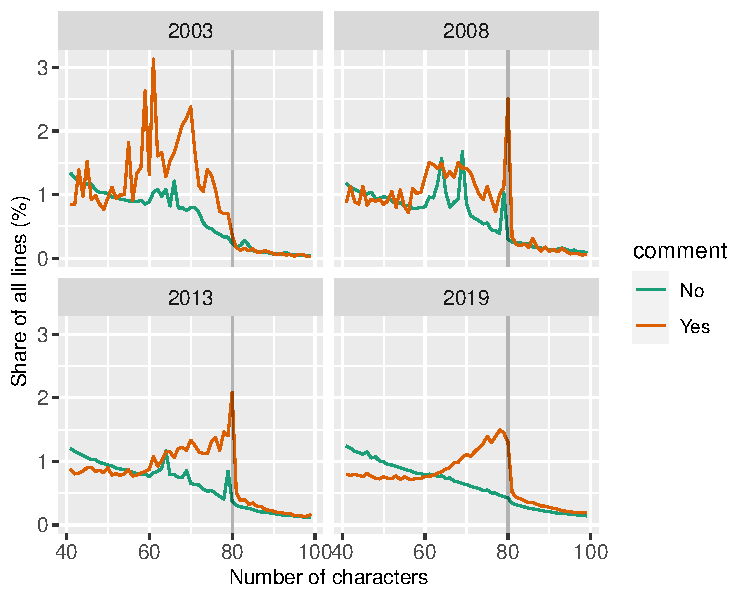
\includegraphics{fig3}
  \caption{Change in line length distribution: 2003, 2008, 2013 and 2019.}
  \label{figure:fig3}
\end{figure}


\subsection{Community-based variations}

Using the aforementioned community detection algorithm of the dependency graph, the largest 20 communities were extracted. These communities are named by their applications. Table~\ref{tab:table2} lists the details of these communities \footnote{``Base packages'' (core packages come with R) such as \CRANpkg{methods} and \CRANpkg{utils} were included in the dependency graph. However, the PSV of recommended packages were not analyzed.}.

Using the naming convention as an example, there are local patterns in PSV (Figure~\ref{figure:fig4}). For example, lower\_snake case is the most popular naming convention in the "RStudio" community as expected because it is the naming convention endorsed by the Tidyverse Style-guide. However, only a few functions exported by the packages from "GUI: Gtk" community uses such convention.

\begin{table}

\caption{\label{tab:table2}The largest 20 communities and their top 3 packages according to PageRank}
\centering
\begin{tabular}[t]{l|r|l}
\hline
Community & Number\_of\_Packages & Top\_3\_Packages\\
\hline
base & 5157 & methods, stats, MASS\\
\hline
RStudio & 4758 & testthat, knitr, rmarkdown\\
\hline
Rcpp & 826 & Rcpp, tinytest, pinp\\
\hline
Statistical Analysis & 463 & survival, Formula, sandwich\\
\hline
Machine Learning & 447 & nnet, rpart, randomForest\\
\hline
Geospatial & 367 & sp, rgdal, maptools\\
\hline
GNU gsl & 131 & gsl, expint, mnormt\\
\hline
Graph & 103 & graph, Rgraphviz, bnlearn\\
\hline
Text Analysis & 79 & tm, SnowballC, NLP\\
\hline
GUI: Tcl/Tk & 55 & tcltk, tkrplot, tcltk2\\
\hline
Infrastructure & 54 & rsp, listenv, globals\\
\hline
Numerical Optimization & 51 & polynom, magic, numbers\\
\hline
Genomics & 43 & Biostrings, IRanges, S4Vectors\\
\hline
RUnit & 38 & RUnit, ADGofTest, fAsianOptions\\
\hline
Survival Analysis & 33 & kinship2, CompQuadForm, coxme\\
\hline
Sparse Matrix & 32 & slam, ROI, registry\\
\hline
GUI: Gtk & 31 & RGtk2, gWidgetstcltk, gWidgetsRGtk2\\
\hline
Bioinformatics & 29 & limma, affy, marray\\
\hline
IO & 28 & RJSONIO, Rook, base64\\
\hline
rJava & 27 & rJava, xlsxjars, openNLP\\
\hline
\end{tabular}
\end{table}

\begin{figure}[htbp]
  \centering
  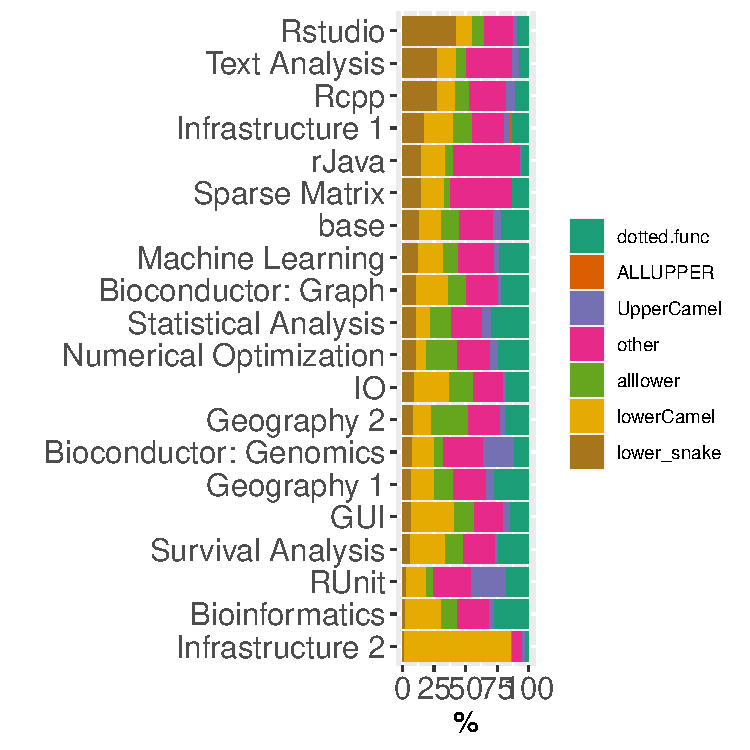
\includegraphics{fig4}
  \caption{Community-specific distribution of naming conventions among 20 large communities.}
  \label{figure:fig4}
\end{figure}

For the binary style-elements, local patterns are also observed (Figure~\ref{figure:fig5}). The most salient pattern is the exceptional high usage of tab indentation in "rJava" and "Bioinformatics" communities, probably due to influences from Java or Perl. Also, packages in "GUI: Gtk" have an exceptional high usage of open curly on its own line.

\begin{figure}[htbp]
  \centering
  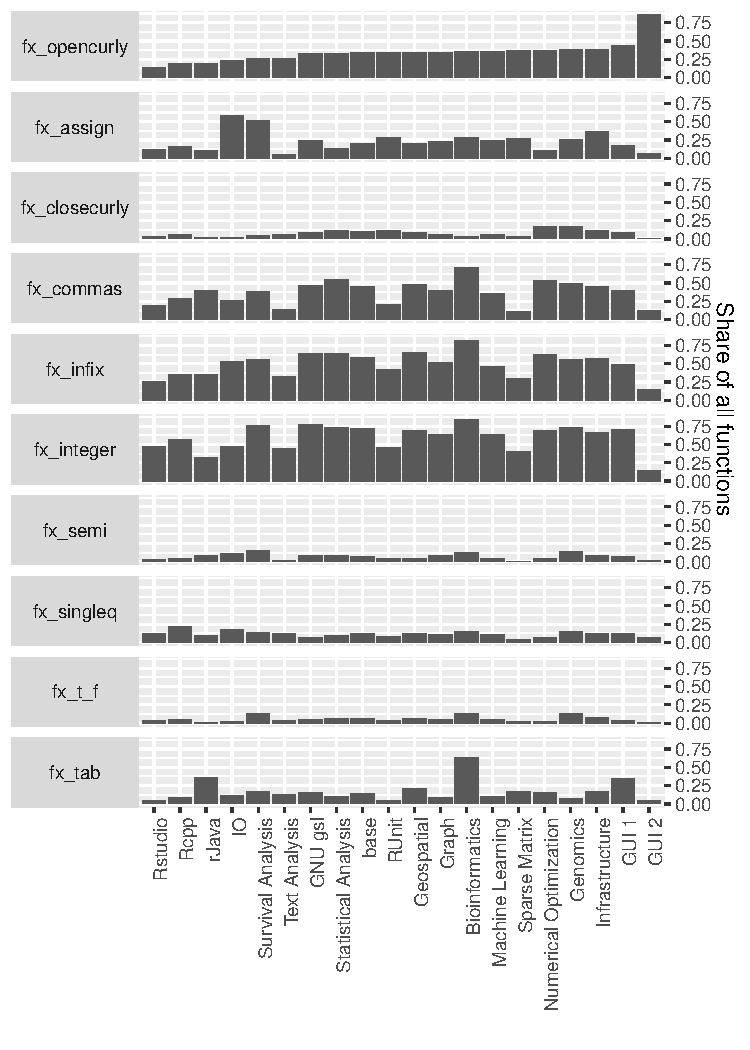
\includegraphics{fig5}
  \caption{Community-specific distribution of style-elements among 20 large communities}
  \label{figure:fig5}
\end{figure}

\subsection{Within-package variations}

The result shows that the consistency of style elements within a package varies (Figure~\ref{figure:fig6}). For example, style elements like fx\_integer, fx\_commas, fx\_infix, fx\_opencurly, and fx\_name have less consistency within a package than fx\_tab, fx\_semi, fx\_t\_f, fx\_closecurly, fx\_singleq, and fx\_assign. This finding echoes previous concerns e.g. \citet{oman, elish, wang, gillespie2016efficient} that these inconsistent style variations within a software project (e.g. in an R package) might make open source collaboration difficult.

\begin{figure}[htbp]
  \centering
  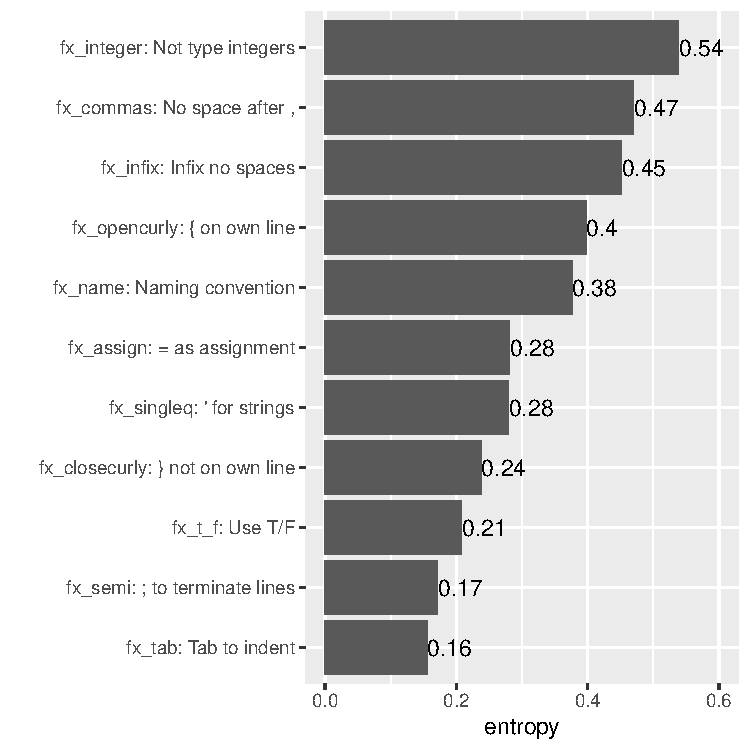
\includegraphics{fig6}
  \caption{Average package-level entropy of 12 style elements}
  \label{figure:fig6}
\end{figure}

In Figure~\ref{figure:fig7}, we contextualize the above analysis by showing the distribution of fx\_name in 20 R packages with the highest PageRank \citep{page1999pagerank} in the CRAN dependency graph. Many of these packages have only 1 dominant naming convention (e.g. lower\_snake or lowerCamel), but not always. For instance, functions with 6 different naming conventions can be found in the package \CRANpkg{Rcpp}.

\begin{figure}[htbp]
  \centering
  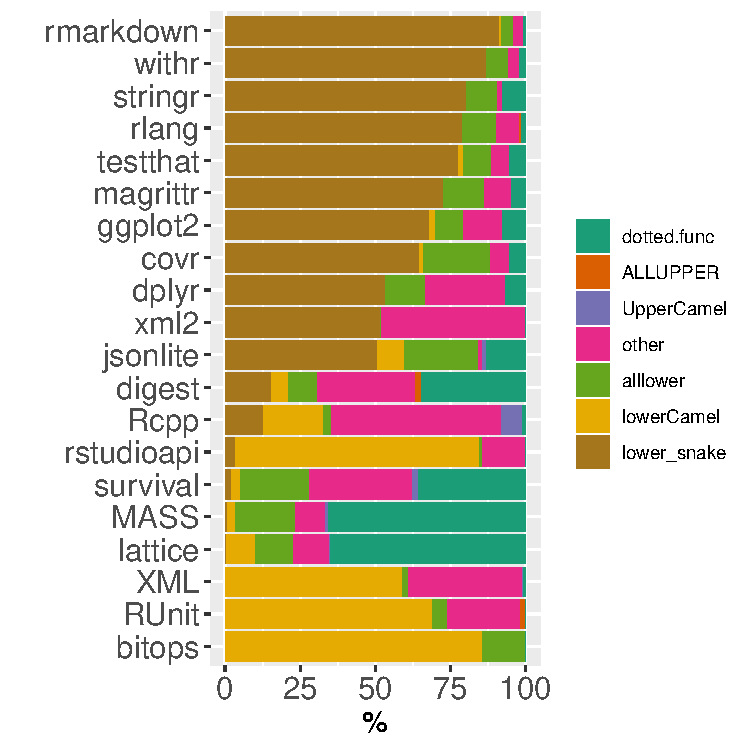
\includegraphics{fig7}
  \caption{Package-specific distribution of naming conventions among the most important packages}
  \label{figure:fig7}
\end{figure}

\section{Discussion}

In this study, we study the PSV in 21 years of CRAN packages across two dimensions: 1) temporal dimension: the longitudinal changes in popularity of various style-elements over 21 years, and 2) cross-sectional dimension: the variations among communities of the latest snapshot of all packages from 1998 to 2019. From our analysis, we identify three factors that possibly drive PSV: the effect of style-guides (trending of naming conventions endorsed by \citet{tidyverse} and \citet{google}), the effect of introducing a new language feature (trending of = usage as assignments after 2001), and the effect of editors (the dominance of 80-character line limit).

From a policy recommendation standpoint, our study provides important insight for the R Development Core Team and other stakeholders to improve the current situation of PSV in R. First, the introduction of a new language feature can have a very long-lasting effect on PSV. "Assignments with the = operator" is a feature that introduced by the R Development Core Team to ``increase compatibility with S-Plus (as well as with C, Java, and many other languages)'' \citep{chambers}. This might be a good intention but it has an unintended consequence of introducing a very persistent PSV that two major style-guides, \citet{tidyverse} and \citet{google}, consider as a bad style.

Second, style-guides, linters, and editors are important standardizers of PSV. Although we have not directly measured the use of style-guides, linters, and editors in our analysis \footnote{The usage of style-guides, linters, and editors cannot be directly measured from the record on CRAN. The maintainers usually do not explicitly state the style-guide they endorsed in their code. Similarly, packages that have been processed with linters do not import or suggest linters such as \CRANpkg{lintr}, \CRANpkg{styler} or \CRANpkg{goodpractice}. It might be possible to infer the use of a specific editor such as RStudio in the development version of a package with signals such as the inclusion of an RStudio Project file. These signals, however, were usually removed in the CRAN submission of the package. Future research should use alternative methods to measure the usage of these 3 things in R packages. In this study, similar to other studies, e.g. \citet{bafatakis:2019:PCS}, we use style compliance as a proxy to usage of a particular style guide, linter or editor.}, we infer their effect by studying the time trend (Figure~\ref{figure:fig1}). Even with these standardizers, programming styles are slow to change. As indicated by the local PSV patterns, we found in some communities, some package developers have their own style. Having said so, we are not accusing those developers of not following the trendy programming styles. Instead, they follow the mantra of ``if it ain't broke don't fix it''. Again, from a policy recommendation standpoint, the existence of local PSV patterns suggests there are many blind spots to the previous efforts in addressing PSV. The authors of the style guides may consider community outreach to promote their endorsed styles, if they want other communities to adopt their styles.

Our analysis also opens up an open question: should R adopt an official style-guide akin the PEP-8 of the Python Software Foundation \citep{vanrossum}? There are of course pros and cons of adopting an official style-guide. As written by \citet{christiansen}, ``style can easily become a religious issue.'' It is not our intention to meddle in this ``religious issue.'' If such an effort would be undertaken by someone else, the following consensus-based style could be used as the basis. The following is an example of a function written in such style.

\begin{example}
softplus_func <- function(value, leaky = FALSE) {
    if (leaky) {
        warnings("using leaky RELU!")
        return(ifelse(value > 0, value, value * 0.01))
    }
    return(log(1 + exp(value)))
}
\end{example}

In essence,

\begin{itemize}
  \item Use snake case
  \item Use <- to assign, don't use =
  \item Add a space after commas
  \item Use TRUE / FALSE, don't use T / F
  \item Put open curly bracket on same line then a newline
  \item Use double quotation mark for strings
  \item Add spaces around infix operators
  \item Don't terminate lines with semicolon
  \item Don’t explicitly type integers (i.e. 1L)
  \item Put close curly bracket on its own line
  \item Don't use tab to indent
\end{itemize}

We must stress here that this \emph{consensus-based} style is only the most popular style based on our analysis, i.e. the \emph{Zeitgeist} (the spirit of the age) \footnote{In 2019, 5.35\% of all functions are in this \emph{Zeitgeist} style. Using electoral system as an analogy, this style is having the plurality (have the highest number of votes) but not the absolute majority (have over 50\% of the votes)}. We have no guarantee that this style can improve clarity or comprehensibility. As a final remark: although enforcing a consistent style can improve open source collaboration \citep{wang}, one must also bear in mind that these rules might need to be adjusted sometimes to cater for programmers with special needs. For example, using spaces instead of tabs for indentation can make code inaccessible to visually impaired programmers \citep{mosal}.

\section{Reproducibility}

The data and scripts to reproduce the analysis in this paper are available at \url{https://github.com/chainsawriot/rstyle}. An archived version is available at this DOI: \url{http://doi.org/10.5281/zenodo.4026589}.

\section{Acknowledgment}

The authors would like to thank Wush Wu and Liang-Do Wang for their valuable comments that greatly improved this paper. Taiwan R User group, R-Ladies Taipei, and attendees of UseR! 2019 gave us thought-provoking feedbacks on this research.

\bibliography{RJreferences}

\newpage
\address{Chia-Yi Yen\\
  Mannheim Business School, Universit\"at Mannheim\\
  L 5, 6, 68131 Mannheim\\
  Germany\\
  \url{https://orcid.org/0000-0003-1209-7789}\\
  \email{yen.chiayi@gmail.com}}

\address{Mia Huai-Wen Chang\\
  Akelius Residential Property AB\\
  Erkelenzdamm 11-13, 10999 Berlin\\
  Germany\\
  \email{mia5419@gmail.com}}

\address{Chung-hong Chan\\
  Mannheimer Zentrum f\"ur Europ\"aische Sozialforschung, Universit\"at Mannheim\\
  A5, 6,  68159 Mannheim\\
  Germany\\
  \url{https://orcid.org/0000-0002-6232-7530}\\
  \email{chung-hong.chan@mzes.uni-mannheim.de}}

